% 图 1 首图：跨栏，由 manuscript_zh.tex 以 \twocolumn[{...}] 置于标题下方。
% 选定设计与当前主表结果（2026-11-04）：figures/Fig1/INDEX.md。
\begin{center}
\captionsetup{type=figure}
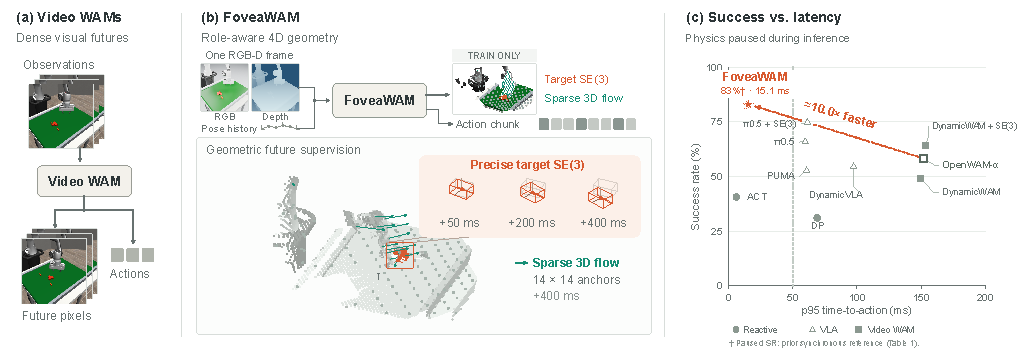
\includegraphics[width=\textwidth]{figures/Fig1/fig1.pdf}
\captionof{figure}{\textbf{\ours 按任务角色分配预测精度。}(a) 用参考录制展示稠密视频未来预测及动作输出的表示形式。(b) \ours 以一帧 RGB-D 和位姿历史为条件，目标 SE(3) 与稀疏 3D 流只用于训练监督，部署时输出动作块。RGB 图为录制状态的 Blender 渲染示意；深度与点云使用录制观测。未来几何展示真实监督标签。流在 \cfgContextGrid{} 网格上采样；箭头表示放大 $3\times$ 的 400\,ms 位移。下方位姿字形展示 $+50$、$+200$ 和 $+400$\,ms 时的目标。(c) 表~\ref{tab:main} 的 Paused 成功率（推理期间暂停物理）与原生 p95 出动作时间。虚线标记 50\,ms。\ours 星形点采用表中的83\%$^{\dagger}$与实测15.1\,ms，相对 OpenWAM-$\alpha$（151.7\,ms）加速约$10.0\times$。$^{\dagger}$Paused 数值沿用表~\ref{tab:main} 选定的先前同步参考结果。}
\label{fig:teaser}
\end{center}
